\ffigbox[\FBwidth]{%
\caption{\centering Graphe avec couplage \(\{be, ci, hp\}\) précalculé}\label{Fig:exam_blanc_ex_3_1}
}{
    \fbox{
        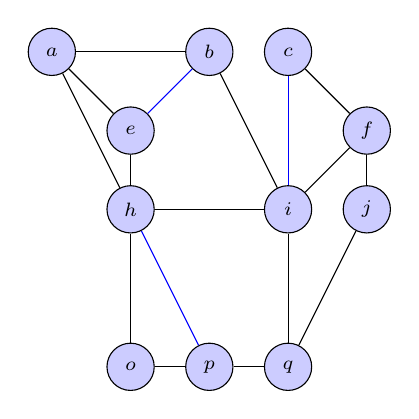
\begin{tikzpicture}[scale=1, main node/.style={circle, draw, fill=blue!20, inner sep=1pt, font=\scriptsize, minimum size=6mm}]
            % les sommets initiaux
            \node[main node] (a) at (-2,2) {\(a\)};
            \node[main node] (b) at (0,2) {\(b\)};
            \node[main node] (c) at (1,2) {\(c\)};

            \node[main node] (e) at (-1,1) {\(e\)};
            \node[main node] (f) at (2,1) {\(f\)};

            \node[main node] (h) at (-1,0) {\(h\)};
            \node[main node] (i) at (1,0) {\(i\)};
            \node[main node] (j) at (2, 0) {\(j\)};

            \node[main node] (o) at (-1, -2) {\(o\)};
            \node[main node] (p) at (0, -2) {\(p\)};
            \node[main node] (q) at (1, -2) {\(q\)};

            % les aretes
            \draw[] (a) -- (b);
            \draw[] (a) -- (e);
            \draw[] (a) -- (h);

            \draw[draw=blue] (b) -- (e);
            \draw[] (b) -- (i);

            \draw[] (c) -- (f);
            \draw[draw=blue] (c) -- (i);
            \draw[] (e) -- (h);

            \draw[] (f) -- (i);
            \draw[] (f) -- (j);

            \draw[] (h) -- (i);
            \draw[] (h) -- (o);
            \draw[draw=blue] (h) -- (p);

            \draw[] (i) -- (q);

            \draw[] (j) -- (q);

            \draw[] (o) -- (p);

            \draw[] (p) -- (q);
        \end{tikzpicture}
    }
}